\documentclass[10pt]{article}
\usepackage{pgfplots}
\pgfplotsset{compat=1.15}
\usepackage{mathrsfs}
\usetikzlibrary{arrows}
\pagestyle{empty}
\begin{document}
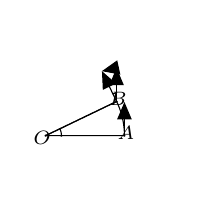
\begin{tikzpicture}[line cap=round,line join=round,>=triangle 45,x=1cm,y=1cm]
\clip(-0.22880265415454426,-0.6364552125121979) rectangle (1.8056675979970274,1.3707676701909202);
\draw [shift={(0,0)},line width=0.4pt]  (0,0) --  plot[domain=0:0.44850383306592945,variable=\t]({1*1*cos(\t r)+0*1*sin(\t r)},{0*1*cos(\t r)+1*1*sin(\t r)}) -- cycle ;
\draw [line width=0.4pt] (0,0)-- (0.9,0.43309);
\draw [shift={(0,0)},line width=0.4pt]  plot[domain=0:0.4485038330659295,variable=\t]({1*0.2*cos(\t r)+0*0.2*sin(\t r)},{0*0.2*cos(\t r)+1*0.2*sin(\t r)});
\draw [->,line width=0.4pt] (0.9,0.43309) -- (0.7144227998047874,0.8187361247678112);
\draw [->,line width=0.4pt] (1,0) -- (1,0.42619219597768815);
\draw [->,line width=0.4pt] (0.9,0.43309) -- (0.9,0.8592821959776882);
\draw [shift={(0.9,0.43309)},line width=0.4pt]  plot[domain=1.5707963267948966:2.0193001598608262,variable=\t]({1*0.1066329020129324*cos(\t r)+0*0.1066329020129324*sin(\t r)},{0*0.1066329020129324*cos(\t r)+1*0.1066329020129324*sin(\t r)});
\draw [->,line width=0.4pt] (0.9,0.8592821959776882) -- (0.7144227998047874,0.8187361247678112);
\begin{scriptsize}
\draw [fill=black] (0,0) circle (0.2pt);
\draw[color=black] (-0.044882910377449056,-0.03360716346505101) node {$O$};
\draw [fill=black] (1,0) circle (0.2pt);
\draw[color=black] (1.0177644981124345,0.0390524883975053) node {$A$};
\draw [fill=black] (0.9,0.43309) circle (0.2pt);
\draw[color=black] (0.9178574768014196,0.47273978545213824) node {$B$};
\draw [fill=black] (0.2,0) circle (0.2pt);

\end{scriptsize}
\end{tikzpicture}
\end{document}